\section{설계}
\label{sec:ldu}

%$$$$$$$$$$$$$$$$$$$$$$$$$$$$$$$$$$$$$$$$$$$$$$$$$$$$$$$$$$$$$$$$$$$$$$$$$$$$$$$$
%Paragraph 1: LDU의 특징을 간단한 설명과 이번장에 대한 설명(LDU의 특징을 요약하여 설명)
%$$$$$$$$$$$$$$$$$$$$$$$$$$$$$$$$$$$$$$$$$$$$$$$$$$$$$$$$$$$$$$$$$$$$$$$$$$$$$$$$

%The \LDU is a log-based concurrent update method to remove scalability
%bottlenecks for the update-heavy data structure.
%The \LDU further improves the performance scalability for update-heavy data
% structures by eliminating the synchronized time-stamp management overhead from previous
%research. One additional advantage of using the \LDU is that it reuses the log
%slots already allocated and used by preceding operations.
%The previous research using the synchronized time-stamp counters method may incur
%time-stamp merging and ordering overhead.
%The \LDU can solve these sequential processing by using two techniques.
%The \LDU instantly removes operation logs at update time that requires time-stamp
%counter and reuses the garbage log instead of creating a new log
%thereby eliminating the synchronized time-stamp counter and cache communication
%bottleneck.
%This section explains these algorithmic design aspects of the \LDU.

LDU는 리눅스 커널의 높은 업데이트 비율을 가진 자료구조의 성능 확장성 문제를 
해결하기 위한 로그 기반 방법 중에 하나이다.
동기화된 타임스탬프 카운터 기반의 퍼코어 로그를 활용한 동시적 업데이트방법은 결국 
타임스탬프 정렬 및 머징 작업을 야기한다.
특히 코어 수가 늘어 날 경우, 퍼코어 로그를 자료 구조에 적용하는 과정에서 추가적인 순차적 프로세싱이 요구된다.
이것은 확장성과 성능을 저해한다. 
이러한 문제를 해결하기 위해, LDU는 로그 기반 방식의 동시적 업데이트 방법과 
원자적 동기화 기능을 최소한으로 이용하도록 설계하였다.
따라서, LDU는 동기화된 타임스탬프 카운터를 사용하는 방식의 타임스탬프를
제거함과 동시에 캐시 커뮤니케이션 오버헤드를 최소화하였다.
이번 장에서는 LDU의 알고리즘적인 디자인 측면에 관해서 설명한다. 

\subsection{접근법(Approach)}


%$$$$$$$$$$$$$$$$$$$$$$$$$$$$$$$$$$$$$$$$$$$$$$$$$$$$$$$$$$$$$$$$$$$$$$$$$$$$$$$$
%Paragraph 2: timestamp가 필요한 이유 : time-sensitive update operation log.
%$$$$$$$$$$$$$$$$$$$$$$$$$$$$$$$$$$$$$$$$$$$$$$$$$$$$$$$$$$$$$$$$$$$$$$$$$$$$$$$$
%The fundamental reason for requiring synchronized time-stamp counters is that
% some operations need to be ordered.
동기화된 타임 스탬프 카운터가 필요한 근본적인 이유는 특정한 명령어들은 반드시 순서가 
지켜져야 한다.
%For example, a process logs an insert operation to the per-core memory, then
%it migrates to another core, and it logs a remove operation, which must
% eventually execute after the insert operation~\cite{SilasBoydWickizerPth}.
예를 들어 프로세스가 삽입 명령어를 퍼코어 메모리에 저장한 후 그 프로세스가 다른 코어로 
이동했을 때, 만약 다음 오퍼레이션이 삭제 오퍼레이션이면 반드시 앞의 삽입 명령어 
다음에 수행하여야 한다~\cite{SilasBoydWickizerPth}. 
%Thus, the synchronized time-stamp counters are needed.
%To specifically explain a time-sensitive log, we use the symbol label used by
%this paper~\cite{Clements15SCR}.
이러한 시간에 민감한 로그를 더 구체적으로 설명하기 위해 우리는 논문 ~\cite{Clements15SCR}에서 
사용한 심볼 방식으로 설명한다.   
%We describe insert as plus-circles $\oplus$, remove as minus-circles
%$\ominus$ and object as color-circles \inv{2}{B}(object B). 
우리는 삽입 명령은 원형으로 된 플러스 모양인 $\oplus$로 표시하고, 삭제 명령은 원형으로된 
마이너스 모양인 $\ominus$으로 표시하고 오브젝트들은 색(\inv{2}{B}(object B))으로 구별하였다.
%Color and vertical offset differentiate cpus.
서로 다른 색깔과 다른 높낮이는 다른 CPU를 의미한다. 
%For example
예를 들어
\begin{center}
$\oplus$\inv{1}{A}, $\oplus$\inv{2}{B}, $\oplus$\inv{3}{C},$\ominus$\inv{2}{A},
$\ominus$\inv{3}{C}, $\oplus$\inv{3}{A}, $\oplus$\inv{3}{C},$\ominus$\inv{1}{C}
\end{center}
%consists of five insert operations, three remove operation, three cpus, and
%three objects.
이것은 5개의 삽입 명령들과 3개의 삭제 명령 그리고 3개의 CPU 그리고 3개의 오브젝트를 의미한다.
%This example shows that $\oplus$\inv{1}{A} and $\ominus$\inv{2}{A},
%time-sensitive logs, must be executed in chronological order.
이 예제에서 $\oplus$\inv{1}{A}와 $\ominus$\inv{2}{A}는 시간에 민감한 로그이며 반드시 시간 순서로
실행되어야 한다.  
%The \LDU can eliminate this time-sensitive logs at update time;as a result, the
% synchronized time-stamp counters are eliminated.
LDU는 이러한 시간에 민감한 명령어들을 업데이트 순간에 삭제한다. 그렇게 함으로써 
동기화된 타임 스탬프 카운터는 제거가 된다.
%One more important fact that these time-sensitive operation logs may be removed
%by optimization phase.
한가지 더 중요한 사실은 이러한 시간에 민감한 로그들은 최적화 단계에서 제거가 된다는 것이다.
%For example, insert-remove operations or remove-insert operations, 
예를 들어, 삽입-삭제 명령어 또는 삭제-삽입 명령어 경우,
%$\oplus$\inv{1}{A}$\ominus$\inv{2}{A}, $\oplus$\inv{3}{C}$\ominus$\inv{3}{C} 
%and $\oplus$\inv{3}{C}$\ominus$\inv{1}{C}, are the cancelable operations before
%a reader, so the remained operation logs, 
$\oplus$\inv{1}{A}$\ominus$\inv{2}{A}, $\oplus$\inv{3}{C}$\ominus$\inv{3}{C} 
그리고 $\oplus$\inv{3}{C}$\ominus$\inv{1}{C}들은 리더가 수행하기 전에
 취소되어도 상관없는 명령어들이다. 
% are the
%cancelable operations before
따라서 남은 로그인 
\begin{center}
 $\oplus$\inv{2}{B}, $\oplus$\inv{3}{A}
\end{center}
로그들은 시간에 민감하지 않은 로그들이다.
%, are non-time-sensitive logs.
%When update operations occur, the \LDU removes these time-sensitive logs using
%the update-side removing technique.
업데이트 명령어가 발생하면 LDU는 이러한 타임 민감한 명령어를 업데이트 측면에서 제거하는 방법을 
사용하여 제거한다.

%$$$$$$$$$$$$$$$$$$$$$$$$$$$$$$$$$$$$$$$$$$$$$$$$$$$$$$$$$$$$$$$$$$$$$$$$$$$$$$$$
%Paragraph 3:  time-sensitive update operation 삭제 방법: Update-side Abosrbing 
%$$$$$$$$$$$$$$$$$$$$$$$$$$$$$$$$$$$$$$$$$$$$$$$$$$$$$$$$$$$$$$$$$$$$$$$$$$$$$$$$

%To remove the time-sensitive log, the \LDU uses the update-side removing
% scheme.
%When insert-remove operations occur in terms of the same object, the scheme
% removes the insert-remove operations at update time.
%The OpLog also optimizes by removing the existing operation rather than
%adding the new one, but the OpLog can not remove log when a thread 
%migrates other core, so it needs additional sequential processing during
%the optimization phase.
%The \LDU, however, has no problem with the migrating other core during logging
%process because it uses the shared atomic swap operation in an individual
% object.

LDU는 시간에 민감한 로그를 제거하기 위해 업데이트 측면에서의 삭제(update-side removing)이라는 방법을 사용한다.
이 방법은 만약 같은 오브젝트(object)에 대해서 삽입(insert)와 삭제(remove)가 발생하였으면, 같은 오브젝트에
대해서, 삽입 명령과 삭제 명령에 대한 로그를 업데이트 시점에 바로 삭제하는 방법이다. 
동기화된 타임 스탬프 카운터(syncronized timestamp counters) 기반의 OpLog도 이러한 로그 삭제 방법 수행하여
최적화를 하였으나, 명령어에 대한 로그가 서로 다른 코어에 존재하는 로그 같은 경우에 로그를 반드시 병합한 후
 삭제를 해야 한다.
동기화된 타임 스탬프 카운터 방법은 워크로드에 따라, 최적화를 위해 또 다른
순차적 프로세싱이 요구된다.
하지만 LDU는 개별적 오브젝트(indivisual object)를 대상으로 스왑(swap) 원자적 명령을
사용하여 공유된 로그를 삭제하는 방법을 사용해서 이런 문제가 없다.


%$$$$$$$$$$$$$$$$$$$$$$$$$$$$$$$$$$$$$$$$$$$$$$$$$$$$$$$$$$$$$$$$$$$$$$$$$$$$$$$$
%Paragraph 5: 리눅스의 Update-side removing 수행 방법
%$$$$$$$$$$$$$$$$$$$$$$$$$$$$$$$$$$$$$$$$$$$$$$$$$$$$$$$$$$$$$$$$$$$$$$$$$$$$$$$$
%The update-side removing logs scheme performs an atomic swap operation in an
%individual object for shared memory systems.
%This atomic swap operation allows update operations to atomically remove with
% the previous cancelable log.
%To achieve update-side removing log, 
%first, add the mark field to the individual object
%structure then use it as a status flag. 
%For example, consider the insert-remove operation sequence at the same object.
%The first insert operation marks the mark field and then it logs into the
% queue.
%If the remove operation occur, the \LDU will not logs;it only changes the mark
% field.
%When the reader applies logs, the \LDU applies the logs to the original data
%structure in case of the true value of the mark field.
%The benefit of this update-side removing scheme is twofold:not only it can
%eliminate the time-sensitive operation but also it can cancel the previous
%operation log in the queue.

업데이트 순간 로그를 지우는 방법은 공유 메모리 시스템의 스왑(swap) 명령어를 사용한다.
이를 위해, LDU는 모든 오브젝트에 삽입과 삭제의 마크(mark) 필드를 추가해서 업데이트 시점에 로그를 
삭제하였다. 
예를 들어 만약 같은 오브텍트에 삽입-삭제(insert-remove) 명령이 수행될 경우 처음 삽입 명령어는
삽입에 대한 마크 필드에 표시하고 큐(queue)에 저장한다. 
다음 삭제 명령부터는 로그를 큐에 저장하지 않고 삽입에 표시한 마크 필드에 표시한 값만
원자적으로 지워주는 방식으로 진행된다.
다음으로 LDU는 로그를 적용할 때, 큐안에 로그가 존재하더라도, 마크 필드가 표시된 로그만 
실제로 실행한다.
이것은 스왑이라는 상대적으로 가벼운 연산과 상대적으로 덜 공유하는 개별적인 공유 오브젝트의
마크 필드(mark filed)를 사용해서 시간에 민감한 명령을 제거할 뿐만 아니라, 동시에 실제
명령을 수행하지 않고 로그를 지워주는 효과를 가져주므로 성능이 향상된다. 

%$$$$$$$$$$$$$$$$$$$$$$$$$$$$$$$$$$$$$$$$$$$$$$$$$$$$$$$$$$$$$$$$$$$$$$$$$$$$$$$$
%Paragraph 7: 또 최적화 방법 reusing garbage object : 
%$$$$$$$$$$$$$$$$$$$$$$$$$$$$$$$$$$$$$$$$$$$$$$$$$$$$$$$$$$$$$$$$$$$$$$$$$$$$$$$$

%The second technique, called reusing garbage logs, reuses the garbage log
%instead of creating a new log.
%The garbage log is the log that has been already cancelled by 
%using the update-side removing scheme,
%but it still occupies a slot in the queue.
%For example, consider the insert-remove-insert operations.
%After the second remove operation, the log is remaining in the queue, but it
% has been already cancelled by using update-side removing; hence {\it insert} mark field
%is zero in the queue.
%In this case, the third insert operation reuses the log in the queue instead of 
%creating a new log using the atomic swap, so it can reduce not only the memory
%overhead but also the queuing overhead.

LDU의 또 다른 최적화 기법은 업데이터 시점에 지우는 기능 때문에 취소된 가비지(garbage) 로그를
재활용하는 것이다.
이러한 가비지 로그일 경우 다음 업데이트 명령에 대해서는 해당 로그를 새로 만들어 넣지 않고 기존 로그를
재활용하는 방법이다.
예를 들어 같은 오브젝트에 대해서 삽입-삭제-삽입(insert-remove-insert) 순서로 업데이트가 수행될 경우, 세 번째
삽입 명령어는 큐에 들어가 있지만 업데이트 시점에 지워진 로그이기 때문에 최소 되어 삽입에 대한 마크 필드가
FALSE로 표시된다. 이런 경우가 가비지 오비젝트(garbage object)이다.
이러면, 다음 삽입 명령에 대해서는 새로운 로그를 큐에 다시 넣지 않고, 해당 오브젝트의 마크 필드만
 변경하여 로그를 재활용하는 방법을 사용한다.

%$$$$$$$$$$$$$$$$$$$$$$$$$$$$$$$$$$$$$$$$$$$$$$$$$$$$$$$$$$$$$$$$$$$$$$$$$$$$$$$$
%Paragraph 11: 중간에 한번씩 log를 flush
%$$$$$$$$$$$$$$$$$$$$$$$$$$$$$$$$$$$$$$$$$$$$$$$$$$$$$$$$$$$$$$$$$$$$$$$$$$$$$$$$
%In addition to the update-side removing logs and the reusing garbage logs,
%the \LDU uses the previous research's scheme that periodically applies the
% operation logs to reduce memory usage and to keep the log from growing without end.
%This approach is similar with the method of previous research such as the
% OpLog's batching updates and flat combining(FC)'s combiner thread.
LDU는 로그 때문에 불필요하게 메모리 낭비를 방지하고, 끝없이 증가하는 것을 방지하기 위해 
로그를 주기적으로 시간 순서대로 적용한다. 
따라서 LDU는 주기적으로 로그를 적용함으로 로그가 쌓여서 발생하는 메모리 낭비를 줄인다. 
이것은 OpLog의 배치 업데이트(batching updates)와 Flat combining의 병합 스레드(combiner thread)와
같이, 1개의 스레드가 업데이트 명령을 수행하므로 캐시 지역성(cache locality)이 높아지는 장점을 가진다. 

%$$$$$$$$$$$$$$$$$$$$$$$$$$$$$$$$$$$$$$$$$$$$$$$$$$$$$$$$$$$$$$$$$$$$$$$$$$$$$$$$
%Paragraph 8: LDU의 로그는 두 종류의 queue에 저장할 수 있도록 지원
%$$$$$$$$$$$$$$$$$$$$$$$$$$$$$$$$$$$$$$$$$$$$$$$$$$$$$$$$$$$$$$$$$$$$$$$$$$$$$$$$
%Furthermore, we design a log's queue using both the per-core and the global
% queue to further support various data structures.
%The per-core queue of the \LDU can remove CAS operations, which access global
%head pointer. 
%However, the per-core queue does not properly apply to all data structures
% since it has some drawbacks.
%The per-core queue has a memory overhead, and developers may need
%an additional management code for per-core memory management(see
% section~\ref{sec:linux}).
%To overcome these shortcomings, the \LDU also supports a global queue.
%The global queue of the \LDU is simple and easy to apply, so it can easily use
% any data structure.
%Though global queue can not perfectly remove global CAS operations, it can
%mitigate the cache communication overhead by using update-side removing
%logs and by reusing garbage logs because it reduces the number of inserting the
%queue(see section~\ref{sec:evaluation}-B).
LDU는 보다 다양한 데이터 구조를 지원하기 위해, 퍼코어또는 전역 큐(global queue) 모두 이용할 수 있게 설계하였다.
그 이유는 데이터 구조가 특성에 따라 퍼코어 구조에 적당한 자료구조가 있고,
전역 큐 구조에 적당한 데이터 구조가 있기 때문이다.
먼저 LDU의 퍼코어 큐는 큐에 로그를 저장할 때, 글로벌 헤드(global head) 포인터에 대한 CAS
명령어를 완전히 제거한 장점을 가진다.
LDU의 퍼코어 큐의 대한 단점으로는 시간에 민감한 로그가 제거되었더라도,
앞에서 설명한 예와 같이 남은 로그들인 $\oplus$\inv{2}{B}, $\oplus$\inv{3}{A}는 순서가 바뀔 수 있다.
이러한 경우 트리와 같은 자료구조에는 문제가 없으나, 스택과 같이 남은 명령의
순서도 민감한 자료구조는 사용하지 못하는 문제점이 있다.
또한, 전형적인 퍼코어 큐를 방법의 단점으로 메모리 관리 코드에 대한 복잡도가 증가하고, 
메모리 사용량도 퍼코어에 추가로 할당을 받으므로 증가된다.
이를 보완하기 위해 LDU는 전역 큐도 같이 지원한다.
LDU의 전역 큐의 장점은 굉장히 간단하여 어떠한 자료구조라도 쉽게 적용할 수 있다. 
또한 퍼코어 처럼 글로벌 헤드 포인터에 대한 CAS연산을 완전히 제거하지 못하지만, LDU의 업데이트 시점에 
지우는 방법과 가비지 로그를 재활용하는 방법으로 글로벌 큐에 로그를 저장하는 횟수를 상당히 줄여서, 
캐시 커뮤니케이션 오버헤드를 상당히 줄일 수 있다. 

%$$$$$$$$$$$$$$$$$$$$$$$$$$$$$$$$$$$$$$$$$$$$$$$$$$$$$$$$$$$$$$$$$$$$$$$$$$$$$$$$
%Paragraph 9: log를 저장하는 queue의 종류는 non-blocking queue를 사용
%$$$$$$$$$$$$$$$$$$$$$$$$$$$$$$$$$$$$$$$$$$$$$$$$$$$$$$$$$$$$$$$$$$$$$$$$$$$$$$$$
%The \LDU uses the non-blocking queue regardless of the per-core queue or the
%global queue since it can proceed without any lock.
%Among non-blocking queues, the \LDU uses multiple producers and single consumer
%based non-blocking queue thereby reducing the CAS operations.
%This queue always inserts node where is a first pointer, so it can minimize
%iteration loops because it causes another CAS operation.
%In addition, this queue merely considers single consumer when it applies
%the logs, so it does not need complex algorithms for the remove operation.
%The queue uses atomic swap operation to acquire all operation logs.
LDU는  논블락킹 큐를 이용하여 로깅한다. 그 이유는 전역 또는 퍼코어 락 없이 수행될 수 
있기 때문이다. 
논블락킹 큐 중에 LDU는 헤드 포인터에 대한 CAS 연산을 최대한 줄인 다중 생산자 단일 소비자(multiple producers
and single consumer)에 활용될 수 있는 자료구조를 이용하였다.
이 큐는 다른 논블락킹 리스트들과 다르게, 삽입 명령을 항상 처음 노드에 삽입함에
따라, CAS가 발생하는 횟수를 상대적으로 줄일 수 있다.
게다가 로그를 적용하는 부분에서 단일 소비자(single consumer)만 고려했기 때문에, 
삭제를 위한 복잡한 알고리즘이 필요 없다. 
예를 들어 단일 소비자(single consumer)는 명령 로그 전체를 얻기 위해, 스왑 명령을 사용하여
 헤드 포인터(head pointer)를 널(NULL)로 원자적으로 제거한다. 


\subsection{실행 예}
\begin{figure*}[h]
  \begin{center}
     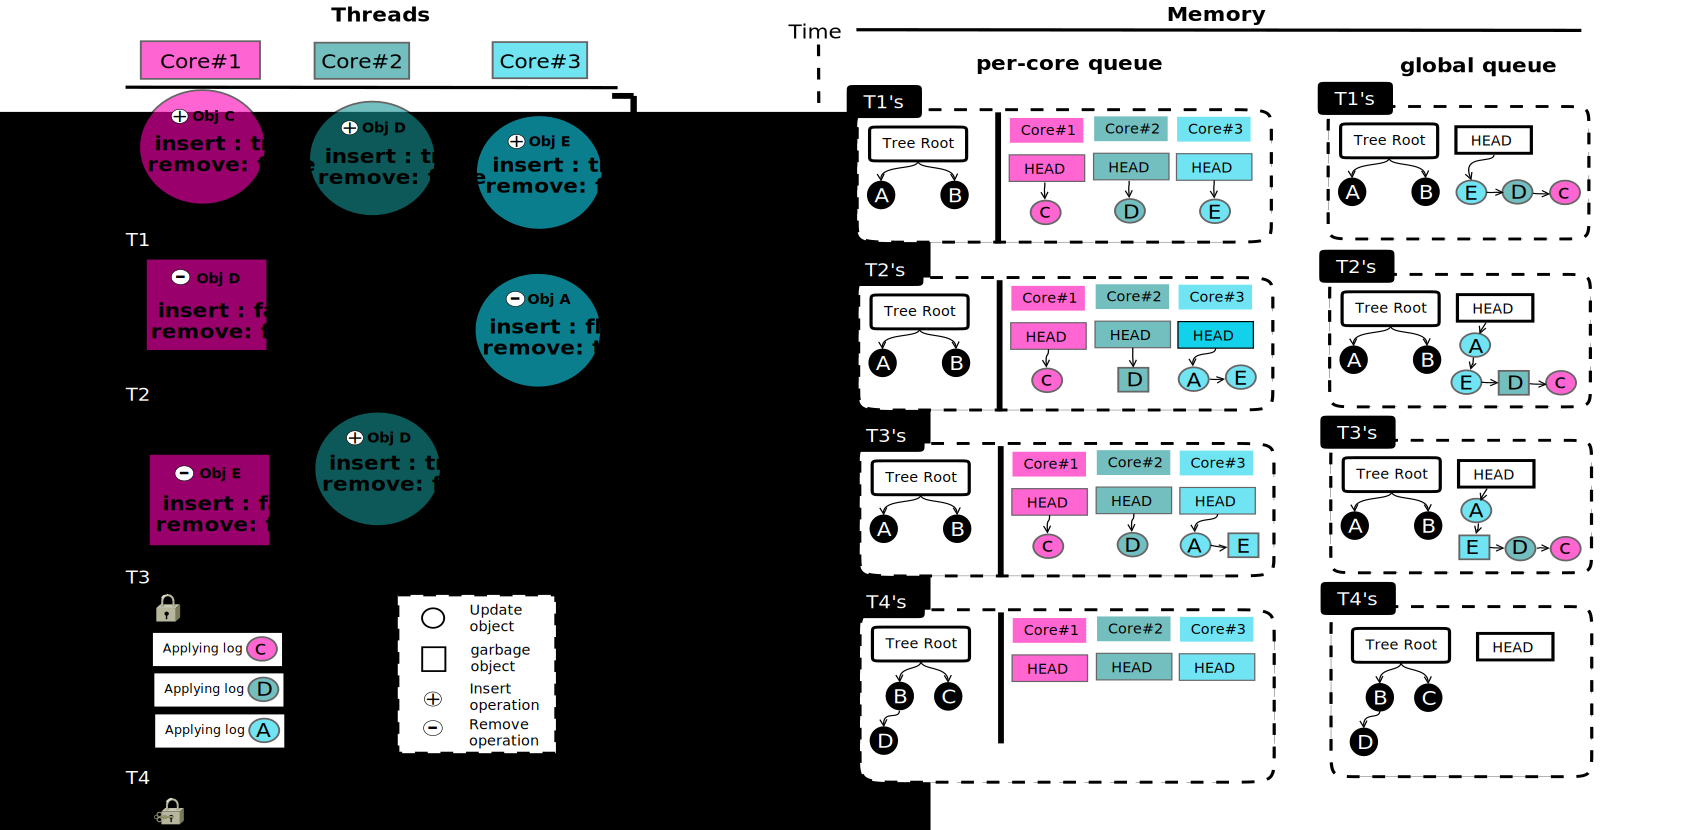
\includegraphics[width=1.0\textwidth,height=0.4\textheight]{fig/basic_gldu}
  \end{center}
  \caption{7개의 업데이트 명령과 1개의 리드 명령에 대한 LDU 예.}
  \label{fig:basic}
\end{figure*}

%$$$$$$$$$$$$$$$$$$$$$$$$$$$$$$$$$$$$$$$$$$$$$$$$$$$$$$$$$$$$$$$$$$$$$$$$$$$$$$$$
%Paragraph 1: Flowchart 구조 설명 
%$$$$$$$$$$$$$$$$$$$$$$$$$$$$$$$$$$$$$$$$$$$$$$$$$$$$$$$$$$$$$$$$$$$$$$$$$$$$$$$$

%Figure \ref{fig:basic} shows an example of the \LDU with a per-core queue and
%a global queue.
그림 \ref{fig:basic}는 LDU가 퍼코어 큐와 전역 큐를 사용하여 수행되는 예를 보여준다.
%In order to explain the concurrent deferred update method for the update-heavy
%data structure, we show how seven update operations can concurrently execute
%without lock before the read operation.
우리는 높은 업데이트 비율을 가지는 자료구조와 함께
 동시적 지연 업데이트 방법을 설명하기 위해서, 7개의 업데이트 명령어가 리드 명령 전에 
 어떻게 동시적으로 수행되는지를 설명한다.
%The update operations sequence is
업데이트 명령어의 순서는 아래와 같다. 
\begin{center}
$\oplus$\inv{1}{C}, $\oplus$\inv{2}{D}, $\oplus$\inv{3}{E},$\ominus$\inv{1}{D},
$\ominus$\inv{3}{A}, $\oplus$\inv{2}{D}, $\ominus$\inv{1}{E}. 
\end{center}.
%To explain the \LDU, we use the previously used symbols with a new garbage
%symbol as rectangle \res{1}{D}.
우리는 LDU를 설명하기 위해서 앞절에서 사용한 심볼에 사각형 모양의 가비지 심볼인 \res{1}{D}를 
추가하여 설명한다. 

%In this figure, execution flows from top to bottom.
이 그림에서 실행 순서는 위에서 부터 아래로 이루어진다.
%The left side of figure shows cpu operations, and the right side of figure
% shows data structures contents at a particular time in a memory.
그림 왼쪽에 있는 것은 CPU의 명령어들을 보여주고 오른쪽에 있는 것은 특정한 시간에 메모리에 있는
자료구조의 내용에 대해서 보여준다. 
%Initially, the tree data structure contains \inv{0}{A} and \inv{0}{B}, and 
%the queue is empty.
초기 트리 자료구조에는 오브젝트 \inv{0}{A}와 \inv{0}{B}가 들어 있고 큐는 비어 있다.
%$$$$$$$$$$$$$$$$$$$$$$$$$$$$$$$$$$$$$$$$$$$$$$$$$$$$$$$$$$$$$$$$$$$$$$$$$$$$$$$$
%Paragraph 2: Flowchart 그림 설명 
%$$$$$$$$$$$$$$$$$$$$$$$$$$$$$$$$$$$$$$$$$$$$$$$$$$$$$$$$$$$$$$$$$$$$$$$$$$$$$$$$
%In the top of figure, \code{Core1}, \code{Core2} and \code{Core3} perform the
%concurrent update operations, $\oplus$\inv{1}{C}, $\oplus$\inv{2}{D} and
%$\oplus$\inv{3}{E}, without lock.
그림의 위쪽에는 \code{Core1}, \code{Core2} 그리고 \code{Core3}은 동시적 업데이트 명령을 수행한다.
따라서 $\oplus$\inv{1}{C}, $\oplus$\inv{2}{D} 그리고 $\oplus$\inv{3}{E}는 락이 없이 동시적으로
수행된다.

%Since the \LDU uses non-blocking queue to save the operation logs, this step
% does not need a update lock, so all threads can be executed in parallel without any lock contention.
LDU는 명령어 로그를 저장하기 위해 논블락킹 큐를 사용하기 때문에, 이 작업에는 업데이트 락이 필요없다.
따라서 모든 쓰레드는 락에 대한 경쟁 없이 동시적으로 수행 가능하다.
%At \code{T1}, the tree contains objects \inv{0}{A} and \inv{0}{B}. 
\code{T1} 시점이 되면, 트리는 오브젝트 \inv{0}{A}과 \inv{0}{B}이 존재한다.
%The per-core queue and the global queue contain $\oplus$\inv{1}{C},
% $\oplus$\inv{2}{D} and $\oplus$\inv{3}{E}, but the logs in the per-core queue are separated.
그리고 퍼코어 큐와 전역 큐는 오브젝트 $\oplus$\inv{1}{C}, $\oplus$\inv{2}{D} 그리고
$\oplus$\inv{3}{E}가 보관되고, 퍼코어 큐는 퍼코어 메모리에 각각 구별되어 저장된다.

%The next operations are $\ominus$\inv{1}{D} and $\ominus$\inv{3}{A}.
다음 명령어들은 $\ominus$\inv{1}{D}과 $\ominus$\inv{3}{A}이며,
%When the $\ominus$\inv{1}{D} operation is executed, the \LDU atomically changes 
%the mark field in the object instead of inserting the queue.
먼저 $\ominus$\inv{1}{D} 명령어가 실행이 되면, LDU는 새롭게 큐에 로그를 넣지 않고, 
원자적으로 오프젝트에 있는 마크 필드를 수정한다. 
%Then, $\ominus$\inv{3}{A} inserts the queue because it is a new operation log.
그리고 $\ominus$\inv{3}{A} 명령어는 새로운 명령어이기 때문에 큐에 바로 저장한다. 
%At \code{T2}, the per-core queue and the global queue contain 
%$\oplus$\inv{1}{C}, $\oplus$\res{2}{D}, $\oplus$\inv{3}{E} and
%$\ominus$\inv{3}{A}.
\code{T2} 시점이 되면, 퍼코어 큐와 전역 큐에는 $\oplus$\inv{1}{C}, $\oplus$\res{2}{D},
$\oplus$\inv{3}{E} 그리고 $\ominus$\inv{3}{A} 로그들이 저장된다. 
%The insert mark field in the object \res{2}{D} is false, called a garbage
% object, has remained in the queue, but it was already canceled 
%by update-side removing logs.
이 시점에서는 오브젝트 \res{2}{D}의 삽입에 대한 마크 필드는 FALSE이다. 
이것은 업데이트 시점에 삭제되는 방법 때문에 취소된 로그이며, 우리는
가비지 오브젝트라 부른다.

%The last operations are $\oplus$\inv{2}{D}, $\ominus$\inv{1}{E}.
마지막 명령어들은 $\oplus$\inv{2}{D}, $\ominus$\inv{1}{E} 이다. 
%The \LDU reuses the log in the queue instead of 
%creating a new log using atomic swap.
LDU는 원자적 스왑을 사용하여 큐에 있는 로그를 새롭게 생성하지 않고 다시 재활용한다. 
%Thus, the object \res{2}{D} changes \inv{2}{D}, and then the object \inv{3}{E} 
%changes \res{3}{E} by performing the update-side removing logs scheme.
그리므로, 업데이트 측면에서 지우는 기술로
 오브젝트 \res{2}{D}는 \inv{2}{D}로 바뀌고, 그리고 오브젝트 \inv{3}{E}는
\res{3}{E}로 바뀐다. 
%At \code{T3}, per-core queue contains
%$\oplus$\inv{1}{C}, $\oplus$\inv{2}{D}, $\ominus$\inv{3}{A} 
%and $\oplus$\res{3}{E}.
\code{T3} 시점이 되면, 퍼코어 큐에는 $\oplus$\inv{1}{C}, $\oplus$\inv{2}{D}, $\ominus$\inv{3}{A} 
그리고 $\oplus$\res{3}{E}가 저장된다. 
%Before the read function, it need to lock the original tree lock using the
%exclusive lock in order to protect the tree operations.
리드 함수가 수행되기 전에 이것은 트리의 명령어를 보호하기 위해서
상호배재 기반의 원본 트리의 락이 필요하다. 
%The \LDU migrates from queue to tree, each of which is the marked object.
LDU는 큐에서 트리로 각각의 명령어를 옮긴다. 이 때 옮길 오브젝트는 마크가 표시된 
오브젝트 로그들이다.
%Thus, $\oplus$\inv{1}{C}, $\oplus$\inv{2}{D} and $\ominus$\inv{3}{A} are
%migrated except for the $\oplus$\res{3}{E} a garbage log.
그러므로, 명령어 $\oplus$\inv{1}{C}, $\oplus$\inv{2}{D} 그리고 $\ominus$\inv{3}{A}
들은 가비지 로그인 $\oplus$\res{3}{E}를 제외하고 옮겨진다. 
%At T5, the tree contains \inv{0}{B}, \inv{0}{C} and
%\inv{0}{D}, so finally, the reader can read eventually consistent data.
T5시점이 되면, 트리는 \inv{0}{B}, \inv{0}{C} 그리고 \inv{0}{D}를 가지게 되어, 
최종적으로 리더는 결국 일관성있는 같은 데이터를 읽게 된다. 

\begin{figure*}[h]
\begin{center}
\inputminted[linenos,fontsize=\footnotesize, tabsize=4]{c}{src/ldu_logical_a.c}
\end{center}
\caption{LDU의 동시적 삽입에 대한 알고리즘.}
\label{fig:gldulogicalupdate}
\end{figure*}


\begin{figure*}[h]
\begin{center}
\inputminted[linenos,fontsize=\footnotesize, tabsize=4]{c}{src/ldu_logical_b.c}
\end{center}
\caption{LDU의 동시적 삽제에 대한 알고리즘.}
\label{fig:gldulogicalupdate}
\end{figure*}


\subsection{알고리즘}

%This section shows skeleton of an algorithm.
%We exclude the log's queue and the \LDU's detailed data structures for
%exposition simplicity.
이번 장은 알고리즘의 중요한 부분에 대해서 보여준다.
우리는 LDU의 로깅하는 큐에 대한 알고리즘과 자세한 자료구조에 대해서는 간략한 설명을 위해 
배제하였다. 

\subsubsection{로그 삽입}
%$$$$$$$$$$$$$$$$$$$$$$$$$$$$$$$$$$$$$$$$$$$$$$$$$$$$$$$$$$$$$$$$$$$$$$$$$$$$$$$$
%Paragraph 1:LDU Concurrent Updates 알고리즘 코드 및 설명 
%$$$$$$$$$$$$$$$$$$$$$$$$$$$$$$$$$$$$$$$$$$$$$$$$$$$$$$$$$$$$$$$$$$$$$$$$$$$$$$$$
%Figure \ref{fig:gldulogicalupdate} shows concurrent update functions.
그림 \ref{fig:gldulogicalupdate}은 동시적 업데이트를 수행하는 함수에 대해 보여준다.
%The concurrent update functions are divided into three phase.
이러한 동시적 업데이트 함수는 3가지 단계로 구분된다.
%The first phase checks this object to see whether or not the
%object is a cancelable object(Line 4, 20).
첫째 단계는 체크단계이며, 이 오브젝트가 취소 가능한 오브젝트인지 확인을 한다(Line 4, 20). 
%When this code is executed, the \code{synchronize} function can
%be invoked by a reader or a periodic timer, so phase 1 needs the atomic
% operation.
이코드가 수행되면, \code{synchronize} 함수는 리더 또는 주기적인 함수에 의해 호출된다.
따라서 첫 번째 단계에서는 원자적 명령어가 필요하다.
%If the corresponding mark field is true, then its mark field is changed to
% false.
만약 그에 상응하는 마크 필드가 TRUE라면 그것에 대한 마크 필드는 FALSE로 수정된다.
%In phase 2 checks this log to see weather or not has already inserted in
%the queue(Line 8, 24).
두 번째 단계에서는 로그가 이미 큐에 들어가 있는 로그인지 아닌지 체크를 수행한다(Line 8, 24).
%If so, because mark field is marked(Line 6, 22), this function directly returns
%true.
만약 그렇다면, 마크 필드는 이미 TRUE로 마크가 됐기 때문에(Line 6, 22), 이 함수는 
바로 종료한다.
%In the last phase, the operation log inserts the non-blocking queue
%when the operation log is the first used log(Line 12, 28).
마지막 단계에서는, 만약 명령어 로그가 처음 사용된 로그라면(Line 12, 28)
 명령어 로그는 논블락킹 큐에 저장된다. 

%$$$$$$$$$$$$$$$$$$$$$$$$$$$$$$$$$$$$$$$$$$$$$$$$$$$$$$$$$$$$$$$$$$$$$$$$$$$$$$$$
%Paragraph 4: 리눅스의 update operation의 특징을 이용한 Update-side Abosrbing 
%$$$$$$$$$$$$$$$$$$$$$$$$$$$$$$$$$$$$$$$$$$$$$$$$$$$$$$$$$$$$$$$$$$$$$$$$$$$$$$$$
%This algorithm is correct because Linux kernel has a unique update
%operations sequence.
이 함수는 항상 옳게 동작한다. 그 이유는 리눅스 커널은 독특한 명령어 순서를 가지고 있기 
때문이다.
%For example, if an insert operation occur, then next operation must be a remove
%operation at the same object because the kernel's update function
%is separated from search, alloc and free functions.
예를 들어, 만약 같은 오브젝트에 대해서 삽입 명령이 발생하면, 다음 명령은 반드시 삭제 명령이 발생한다.
왜냐하면, 리눅스 업데이트 함수는 검색(search), 동적할당(alloc) 그리고 해제(free) 함들들과 
구별되어 있기 때문이다.
%The remove-remove or insert-insert operation in Linux kernel is
%forbidden: if remove-remove operation occur, the second remove operation may
%encounter a crash because this object can be concurrently freed after the first
% remove operation, so we check the corresponding mark field(Line 5, 21).
리눅스 커널의 삭제-삭제 순서 또는 삽입-삽입 명령 순서는 금지된다. 
만약에 삭제-삭제 명령어 순서가 발생하면, 두 번째 삭제 명령어는 크레쉬(crash) 만날 수 있다.
그 이유는 첫 번째 삭제 명령어 다음에 이 오브젝트는 바로 동시에 메모리 해제가 될 수 있기 때문다.
따라서 우리는 그에 상응하는 마크 필드를 점검하였다(Line 5, 21).


\subsubsection{로그 적용}

\begin{figure*}[h]
\begin{center}
\inputminted[linenos,fontsize=\footnotesize, tabsize=4]{c}{src/ldu_physical.c}
\end{center}
%\rule{\columnwidth}{0.5pt}
%\vspace{-\baselineskip}
\caption{로그를 적용하는 알고리즘.}
\label{fig:glduphysicalupdate}
\end{figure*}


%$$$$$$$$$$$$$$$$$$$$$$$$$$$$$$$$$$$$$$$$$$$$$$$$$$$$$$$$$$$$$$$$$$$$$$$$$$$$$$$$
%Paragraph 2:LDU Deferred Updates 알고리즘 코드 및 설명 
%$$$$$$$$$$$$$$$$$$$$$$$$$$$$$$$$$$$$$$$$$$$$$$$$$$$$$$$$$$$$$$$$$$$$$$$$$$$$$$$$

%Figure \ref{fig:glduphysicalupdate} shows deferred update function, which
%applies the operation logs.
그림 \ref{fig:glduphysicalupdate}은 명령어 로그들을 적용하는 지연 업데이트 함수를 보여준다. 
%The \code{synchronize} function is invoked before the read, or it can be
%periodically invoked by the timer handler because of preventing the continuous
%growing the logs.
\code{synchronize} 함수는 리드 전에 호출되거나 주기적으로 호출되는 타이머 핸들러(timer handler)에 의해
호출된다. 
그 이유는 무한정 커지는 로그를 방지하기 위해서이다.
%Before the execution of the \code{synchronize} function, it has been locked by
% using the object lock, so this function proceed with a single consumer thread
%in a way similar to the OpLog's batching updates and FC's combiner thread.
\code{synchronize} 함수가 수행하기 전에, \code{synchronize} 함수는 오브젝트의 락을 사용하여
반드시 락이 걸려 있어야 한다.
따라서 이 함수는 단일 소비자로 수행되어야 한다. 즉 이 방법은 OpLog의 배치
 업데이트(batching updates)와 FC의 컴파이너 쓰레드(combiner thread)와 비슷하다고 볼수 있다. 
%First, the \code{synchronize} function acquires queue's head pointer by using
% atomic swap operation(Line 3).
처음으로 \code{synchronize} 함수는 큐의 헤드 포인터를 원자적인 스왑 명령(Line 3)을 이용하여 
얻는다.
%Because the \LDU periodically applies the logs queue, the \LDU update
% operations may concurrently execute with the \code{synchronize} function.
LDU는 주기적으로 로그의 큐를 적용하기 때문에, LDU의 업데이트 명령어는 \code{synchronize} 함수와 
동시에 수행될 수 있다. 
%Thus, before the applying original data structure, the mark field is
%set to false(Line 8, 9).
그러므로 원본 자료구조에 적용하기 전에 마크필드는 FALSE로 수정된다(Line 8,9).
%The used flag for the garbage log is set to false indicating that the queue
%does not contain this object(Line 10).
가비지 로그를 위한 사용 플래그(used flag)는 FALSE로 수정된다. 이것은 이 오브젝트가 큐에 포함되어 있지 
않는다는 것을 의미한다(Line 10).
%The \code{synchronize} function
%once again checks(Line 12, 13) to see whether the mark field
%is changed between the applying logs(Line 8) and clearing garbage bit(Line
% 10).
\code{synchronize} 함수는 한 번 더 마크 필드가 적용하는 과정(Line 8)과 가비지 비트를 초기화하는 과정(Line
10)에서 수정되었는지 다시 체크를 한다(Line 12,13).

